
\begin{figure}[H]
  \centering 
  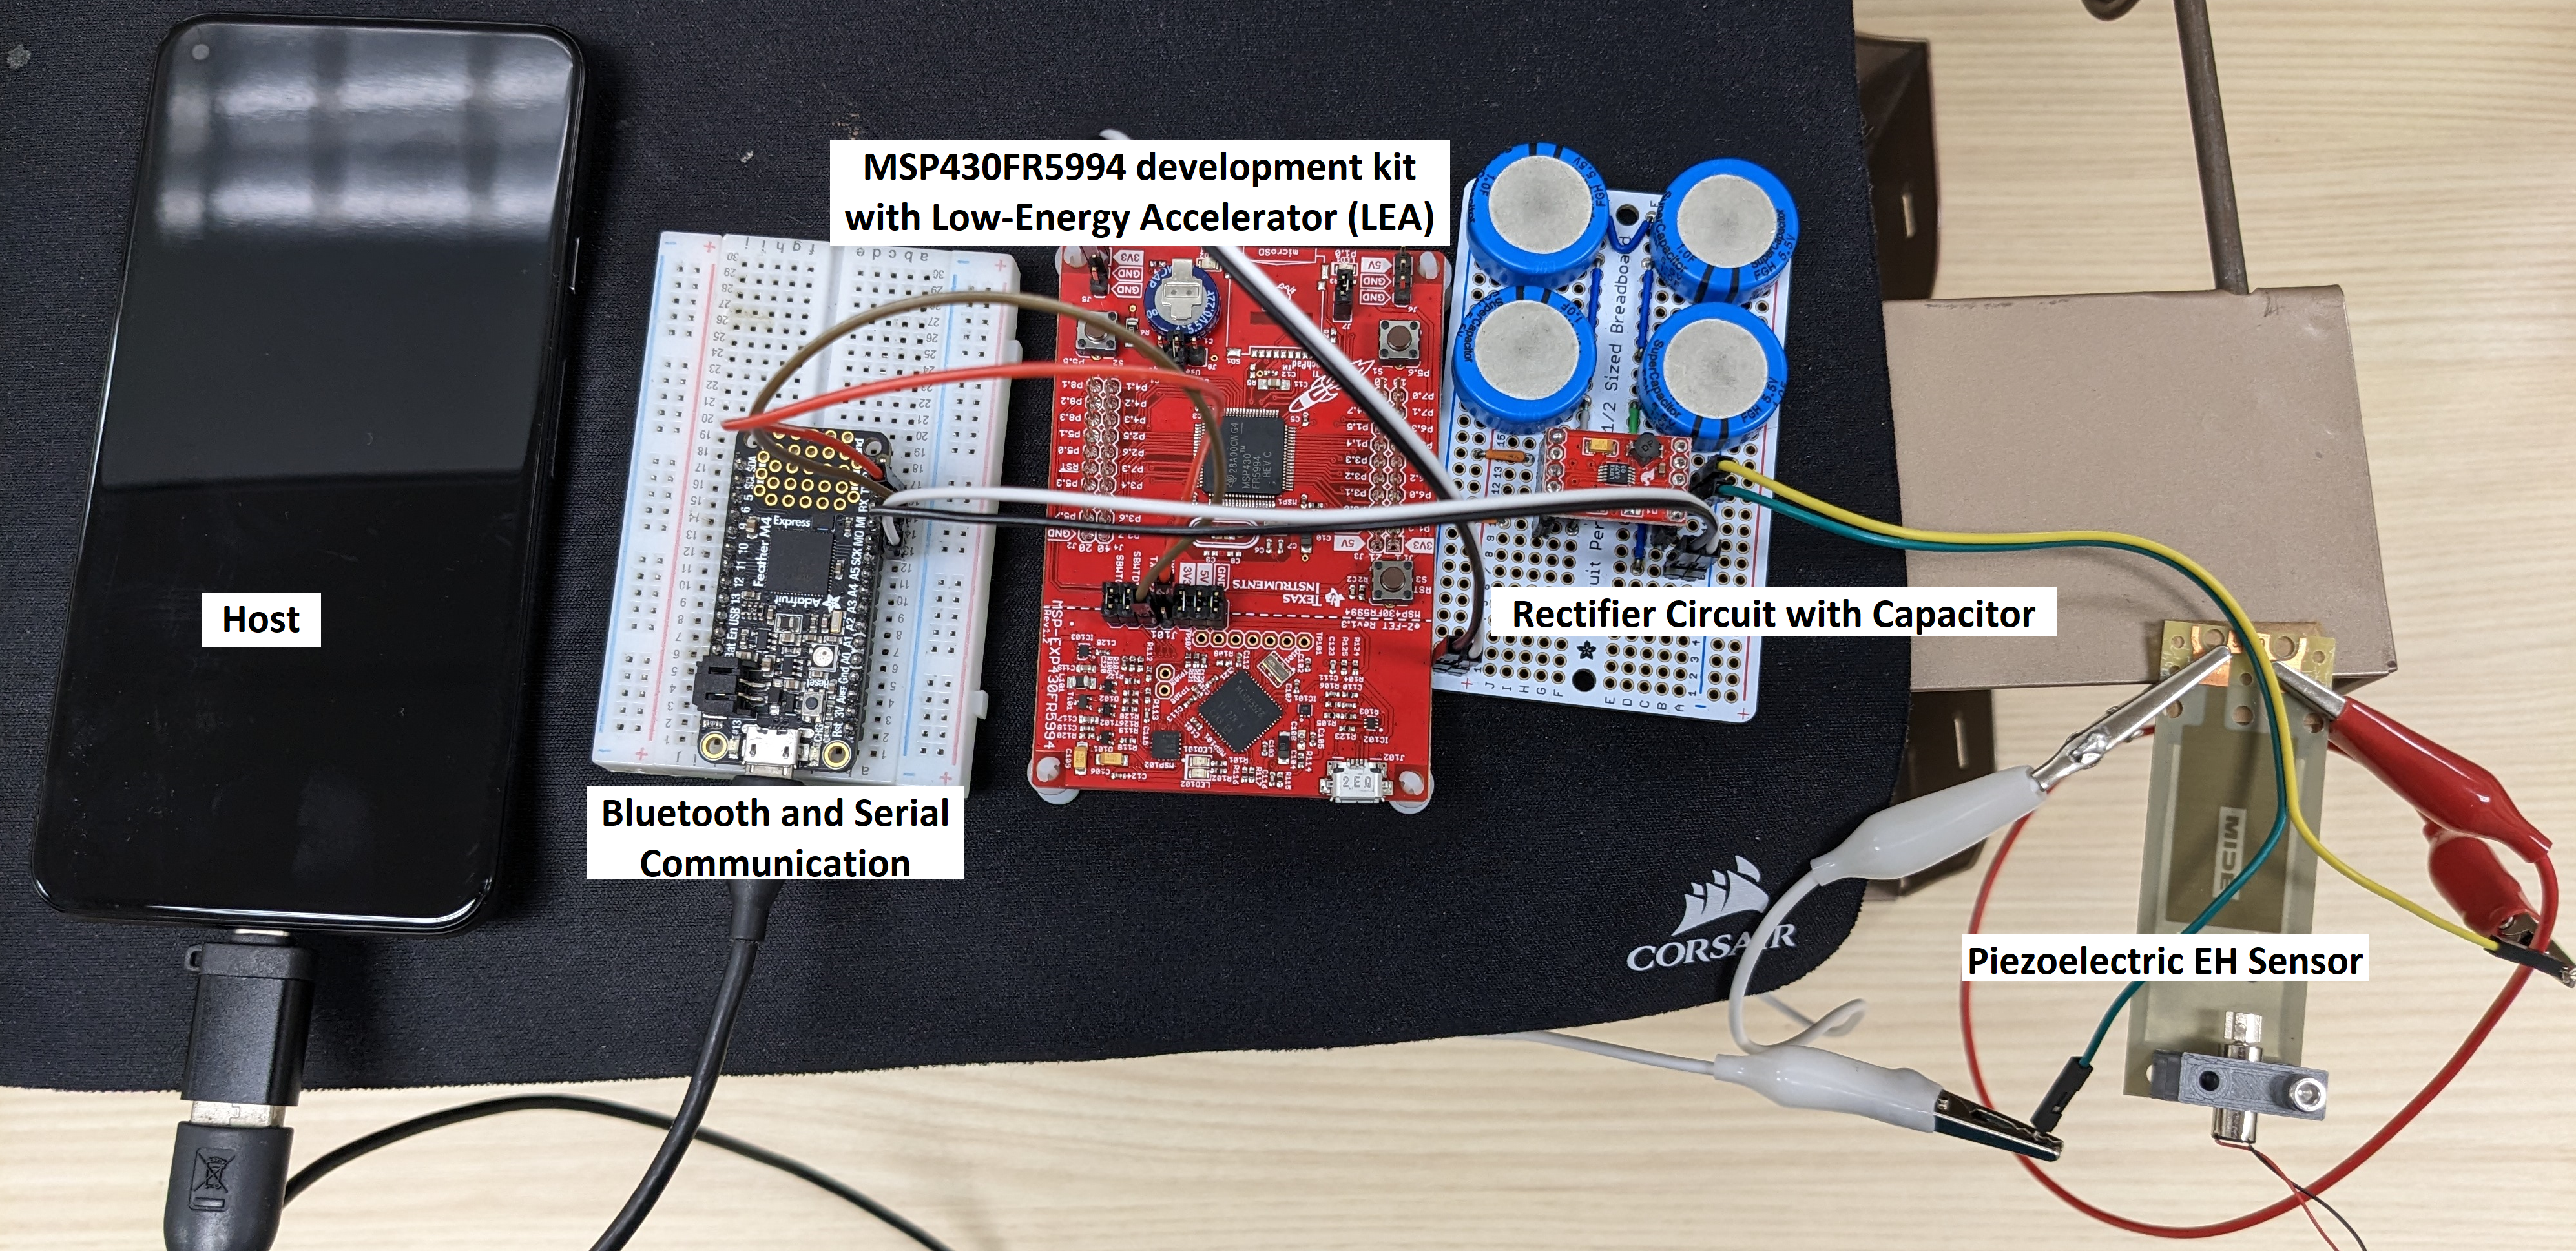
\includegraphics[clip, width=0.5\linewidth]{figs/SeekerCommercial.png}
  \caption{Hardware setup of NExUME using MSP-EXP430FR5994 as the edge compute,   Adafruit ItsyBitsy nRF52840 Express for communicating, Energy Harvester Breakout - LTC3588 with supercapacitors as energy rectification and storage and a Pixel-5 phone as the host.}
  \label{Fig:cotsFIG}
\end{figure}

% Please add the following required packages to your document preamble:
% \usepackage{multirow}
% \usepackage{graphicx}
\begin{table}[H]
\resizebox{\columnwidth}{!}{%
\begin{tabular}{lllllll}
\multicolumn{1}{c}{\multirow{2}{*}{\textbf{Datasets}}} &
  \multicolumn{1}{c}{\multirow{2}{*}{\textbf{Full Power}}} &
  \multicolumn{4}{c}{\textbf{MSP on Piezo}} &
  \textbf{} \\
\multicolumn{1}{c}{} &
  \multicolumn{1}{c}{} &
  \multicolumn{1}{c}{\textbf{AP}} &
  \multicolumn{1}{c}{\textbf{PT}} &
  \multicolumn{1}{c}{\textbf{iNAS+PT}} &
  \multicolumn{1}{c}{\textbf{NExUME}} &
  \textbf{Better} \\
\textbf{FMNIST}     & 98.70 & 71.90 & 79.72 & 83.68 & \textbf{88.90} & 6.24\%  \\
\textbf{CIFAR10}    & 89.81 & 55.05 & 62.00 & 66.98 & \textbf{76.29} & 13.90\% \\
\textbf{MHEALTH}    & 89.62 & 59.76 & 65.40 & 71.56 & \textbf{80.75} & 12.84\% \\
\textbf{PAMAP}      & 87.30 & 57.38 & 65.77 & 65.38 & \textbf{75.16} & 14.97\% \\
\textbf{AudioMNIST} & 88.20 & 67.29 & 73.16 & 75.41 & \textbf{80.01} & 6.10\% 
\end{tabular}%
}
\caption{Accuracy of NExUME on MSP board using vibration from a Piezoelectric harvestor. Better refers to the improvement over iNAS+PT baseline.}
\label{tab:AccMSPonPz}
\end{table}

% Please add the following required packages to your document preamble:
% \usepackage{multirow}
% \usepackage{graphicx}
\begin{table}[H]
\resizebox{\columnwidth}{!}{%
\begin{tabular}{lllllll}
\multicolumn{1}{c}{\multirow{2}{*}{\textbf{Datasets}}} &
  \multicolumn{1}{c}{\multirow{2}{*}{\textbf{Full Power}}} &
  \multicolumn{4}{c}{\textbf{MSP on Thermal}} &
  \textbf{} \\
\multicolumn{1}{c}{} &
  \multicolumn{1}{c}{} &
  \multicolumn{1}{c}{\textbf{AP}} &
  \multicolumn{1}{c}{\textbf{PT}} &
  \multicolumn{1}{c}{\textbf{iNAS+PT}} &
  \multicolumn{1}{c}{\textbf{NExUME}} &
  \textbf{Better} \\
\textbf{FMNIST}     & 98.70 & 80.92 & 86.32 & 88.93 & \textbf{95.62} & 7.53\%  \\
\textbf{CIFAR10}    & 89.81 & 64.78 & 69.29 & 71.53 & \textbf{83.78} & 17.13\% \\
\textbf{MHEALTH}    & 89.62 & 69.77 & 73.99 & 77.70 & \textbf{89.62} & 15.34\% \\
\textbf{PAMAP}      & 87.30 & 66.33 & 71.84 & 74.47 & \textbf{85.24} & 14.46\% \\
\textbf{AudioMNIST} & 88.20 & 73.84 & 78.03 & 81.60 & \textbf{87.64} & 7.40\% 
\end{tabular}%
}
\caption{Accuracy of NExUME on MSP board using thermocouple based thermal harvester. Better refers to the improvement over iNAS+PT baseline.}
\label{tab:AccMSPonTh}
\end{table}

% Please add the following required packages to your document preamble:
% \usepackage{multirow}
% \usepackage{graphicx}
\begin{table}[H]
\resizebox{\columnwidth}{!}{%
\begin{tabular}{lllllll}
\multicolumn{1}{c}{\multirow{2}{*}{\textbf{Datasets}}} &
  \multicolumn{1}{c}{\multirow{2}{*}{\textbf{Full Power}}} &
  \multicolumn{4}{c}{\textbf{Arduino on RF}} &
  \textbf{} \\
\multicolumn{1}{c}{} &
  \multicolumn{1}{c}{} &
  \multicolumn{1}{c}{\textbf{AP}} &
  \multicolumn{1}{c}{\textbf{PT}} &
  \multicolumn{1}{c}{\textbf{iNAS+PT}} &
  \multicolumn{1}{c}{\textbf{NExUME}} &
  \textbf{Better} \\
\textbf{FMNIST}     & 98.70 & 74.44 & 79.63 & 83.61 & \textbf{90.44} & 8.17\%  \\
\textbf{CIFAR10}    & 89.81 & 58.11 & 63.91 & 65.01 & \textbf{79.60} & 22.44\% \\
\textbf{MHEALTH}    & 89.62 & 63.52 & 67.40 & 74.30 & \textbf{83.86} & 12.87\% \\
\textbf{PAMAP}      & 87.30 & 61.39 & 67.24 & 69.45 & \textbf{77.00} & 10.87\% \\
\textbf{AudioMNIST} & 88.20 & 66.11 & 74.28 & 76.60 & \textbf{78.87} & 2.97\% 
\end{tabular}%
}
\caption{Accuracy of NExUME on Arduino nano board using WiFi based RF harvester. Better refers to the improvement over iNAS+PT baseline.}
\label{tab:AccARDonRF}
\end{table}

% Please add the following required packages to your document preamble:
% \usepackage{multirow}
% \usepackage{graphicx}
\begin{table}[H]
\resizebox{\columnwidth}{!}{%
\begin{tabular}{lllllll}
\multicolumn{1}{c}{\multirow{2}{*}{\textbf{Datasets}}} &
  \multicolumn{1}{c}{\multirow{2}{*}{\textbf{Full Power}}} &
  \multicolumn{4}{c}{\textbf{Arduino on Thermal}} &
  \textbf{} \\
\multicolumn{1}{c}{} &
  \multicolumn{1}{c}{} &
  \multicolumn{1}{c}{\textbf{AP}} &
  \multicolumn{1}{c}{\textbf{PT}} &
  \multicolumn{1}{c}{\textbf{iNAS+PT}} &
  \multicolumn{1}{c}{\textbf{NExUME}} &
  \textbf{Better} \\
\textbf{FMNIST}     & 98.70 & 77.04 & 80.44 & 83.08 & \textbf{89.90} & 8.20\%  \\
\textbf{CIFAR10}    & 89.81 & 60.38 & 65.90 & 66.98 & \textbf{80.70} & 20.48\% \\
\textbf{MHEALTH}    & 89.62 & 65.74 & 69.88 & 72.41 & \textbf{85.75} & 18.42\% \\
\textbf{PAMAP}      & 87.30 & 62.76 & 65.93 & 71.46 & \textbf{81.27} & 13.73\% \\
\textbf{AudioMNIST} & 88.20 & 69.12 & 73.86 & 77.79 & \textbf{83.54} & 7.39\% 
\end{tabular}%
}
\caption{Accuracy of NExUME on Arduino nano board using thermocouple based thermal harvester. Better refers to the improvement over iNAS+PT baseline.}
\label{tab:AccARDonTh}
\end{table}


% Please add the following required packages to your document preamble:
% \usepackage{multirow}
% \usepackage{graphicx}
